%%% Поля и разметка страницы %%%
\documentclass[a4paper,12pt]{article}
\usepackage{lscape}		% Для включения альбомных страниц

%%% Кодировки и шрифты %%%
\usepackage{cmap}						% Улучшенный поиск русских слов в полученном pdf-файле
\usepackage[T2A]{fontenc}				% Поддержка русских букв
\usepackage[utf8]{inputenc}				% Кодировка utf8
\usepackage[english, russian]{babel}	% Языки: русский, английский
%\usepackage{pscyr}						% Красивые русские шрифты

%%% Математические пакеты %%%
\usepackage{amsthm,amsfonts,amsmath,amssymb,amscd} % Математические дополнения от AMS

%%% Оформление абзацев %%%
\usepackage{indentfirst} % Красная строка

%%% Цвета %%%
\usepackage[usenames]{color}
\usepackage{color}
\usepackage{colortbl}

%%% Таблицы %%%
\usepackage{longtable}					% Длинные таблицы
\usepackage{multirow,makecell,array}	% Улучшенное форматирование таблиц

%%% Общее форматирование
\usepackage[singlelinecheck=off,center]{caption}	% Многострочные подписи
\usepackage{soul}									% Поддержка переносоустойчивых подчёркиваний и зачёркиваний

%%% Библиография %%%
\usepackage{cite} % Красивые ссылки на литературу

%%% Для многострочных формул gathered
\usepackage{amsmath}

%%% Для прямых, а не наклонных интегралов
\usepackage{wasysym}
\let\int\varint

%%% Гиперссылки %%%
\usepackage[plainpages=false,pdfpagelabels=false]{hyperref}
\definecolor{linkcolor}{rgb}{0.9,0,0}
\definecolor{citecolor}{rgb}{0,0.6,0}
\definecolor{urlcolor}{rgb}{0,0,1}
\hypersetup{
    colorlinks, linkcolor={linkcolor},
    citecolor={citecolor}, urlcolor={urlcolor}
}

%%% Изображения %%%
\usepackage{graphicx}		% Подключаем пакет работы с графикой
\graphicspath{{images/}}	% Пути к изображениям

%%% Выравнивание и переносы %%%
\sloppy					% Избавляемся от переполнений
\clubpenalty=10000		% Запрещаем разрыв страницы после первой строки абзаца
\widowpenalty=10000		% Запрещаем разрыв страницы после последней строки абзаца

%%% Библиография %%%
\makeatletter
\bibliographystyle{utf8gost705u}	% Оформляем библиографию в соответствии с ГОСТ 7.0.5
\renewcommand{\@biblabel}[1]{#1.}	% Заменяем библиографию с квадратных скобок на точку:
\makeatother

%%% Колонтитулы %%%
\let\Sectionmark\sectionmark
\def\sectionmark#1{\def\Sectionname{#1}\Sectionmark{#1}}
\makeatletter
\newcommand*{\currentname}{\@currentlabelname}
\renewcommand{\@oddhead}{\it \vbox{\hbox to \textwidth%
    % {\hfil Фамилия И.О. --- Короткое название черновика\hfil\strut}\hbox to \textwidth%
    {\today \hfil \thesection~\Sectionname\strut}\hrule}}
\makeatother

%%%%%%%%%%%%%%%%%%%%%%%%%%%%%%%%%%%%%%%%%%%%%%%%%%%%%%%%%%%%%%%%%%%%%%%%%%%%%%%%%%%
\begin{document}
\section{Что такое композиты}
Композитный материал -- искуственно созданный материал, обладающий неоднородными физическими свойствами.
В механике деформируемого твёрдого тела таким материалам ставится в соответствие математическая модель, описываемая определяющими соотношениями, вида:

\begin{equation}
    \label{eq:BasicDefRelations}
    \mathfrak{b} = \mathfrak{F}(\mathfrak{a}, \vec{x}),
\end{equation}

где, 
$\mathfrak{a}$ 
может быть, например, градиентом температуры, в случае задачи темплопроводности или тензором деформации, в случае задачи упругости; 
$\mathfrak{b}$ 
будет, соответственно, вектором теплопроводности, либо тензором напряжения; 
$\vec{x}$ 
-- вектор координат.

В выражении 
\ref{eq:BasicDefRelations} 
явно задана зависимость соотношения от координат. 
Определяющие соотношения выражаются через материальные функции.
Примеры материальных функций: тензор упругости, тензор теплопроводности.
Материальные функции являются кусочнонепрерывными и терпят разрыв на границах раздела сред.

% искусственно созданный неоднородный сплошной материал, состоящий из двух или более компонентов с чёткой границей раздела между ними. 

Периодический композитный материал -- композитный материал, материальные функции, которого, периодические по координатам.

\begin{equation}
    \label{eq:BasicPeriodicFuction}
    \mathfrak{F}(\mathfrak{a}, \vec{x} + n_i\vec{a_i}) = \mathfrak{F}(\mathfrak{a}, \vec{x}),
\end{equation}

где, 
$\vec{a_i}$ 
-- постоянные векторы, 
$n_i$ 
-- произвольные числа.

Периодические композитные материалы, по типу периодичности, можно разделить на 3 вида:

1-периодические композитные материалы (слоистые) (рис. 
\ref{images:one_period}
).
Физические свойства изменяются периодически вдоль одного направления (на рис. 
\ref{images:one_period}
направление 
$Ox$
). В доль двух других направлений физические свойства не изменяются.

\begin{equation}
    \begin{array}{ccc}
    \vec{a}_x = \left(\begin{array}{c}h_x\\0\\0\end{array}\right) & 
    \vec{a}_y = \left(\begin{array}{c}0\\0\\0\end{array}\right) & 
    \vec{a}_z = \left(\begin{array}{c}0\\0\\0\end{array}\right)
    \end{array}
\end{equation}

\begin{figure} [ht] 
    \center
    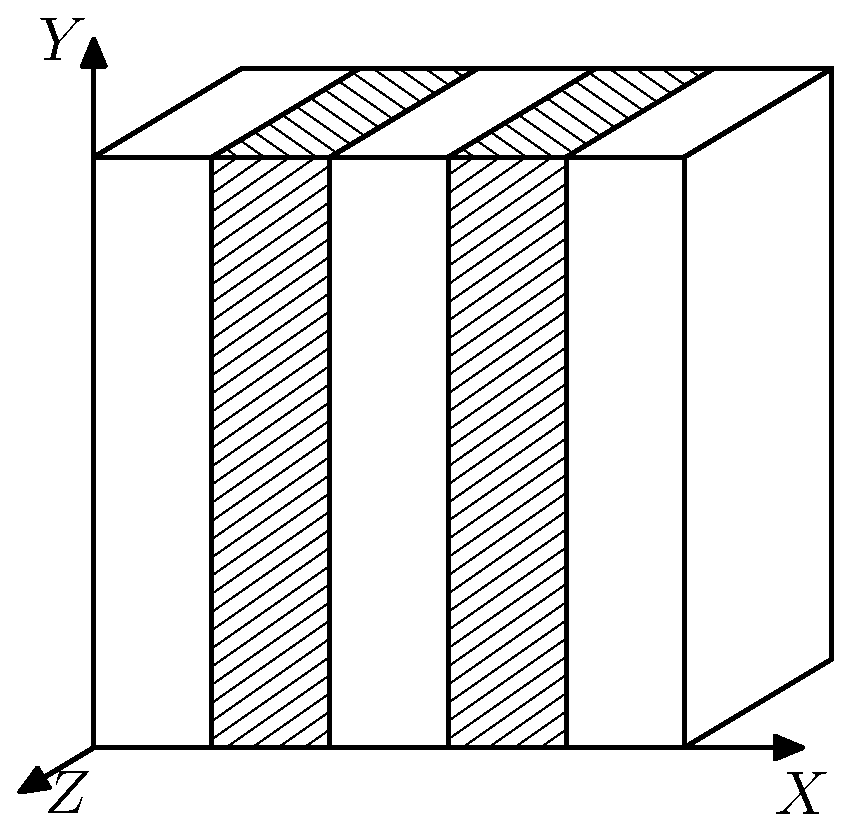
\includegraphics [scale=0.5] {one_period}
    \caption{1-периодчекая среда.} 
    \label{images:one_period}  
\end{figure}
% \begin{figure}[h]
%     \def\svgwidth{1.5\textwidth}%
%     \resizebox{\textwidth}{!}{%
%         \input{num1.tex}%
%     }
%     \caption{Test with ``figure'' environment.}
% \end{figure}

2-периодические коомпозитные материалы (армированные) (рис. 
\ref{images:two_period}
).
Физические свойства изменяются периодически вдоль двух направлений (на рис. 
\ref{images:two_period} $Ox$
и 
$Oy$
).  Вдоль третьего направления 
($Oz$) 
физические свойства не изменяются. 

\begin{equation}
    \begin{array}{ccc}
    \vec{a}_x = \left(\begin{array}{c}h_x\\0\\0\end{array}\right) & 
    \vec{a}_y = \left(\begin{array}{c}0\\h_y\\0\end{array}\right) & 
    \vec{a}_z = \left(\begin{array}{c}0\\0\\0\end{array}\right)
    \end{array}
\end{equation}

\begin{figure} [ht] 
    \center
    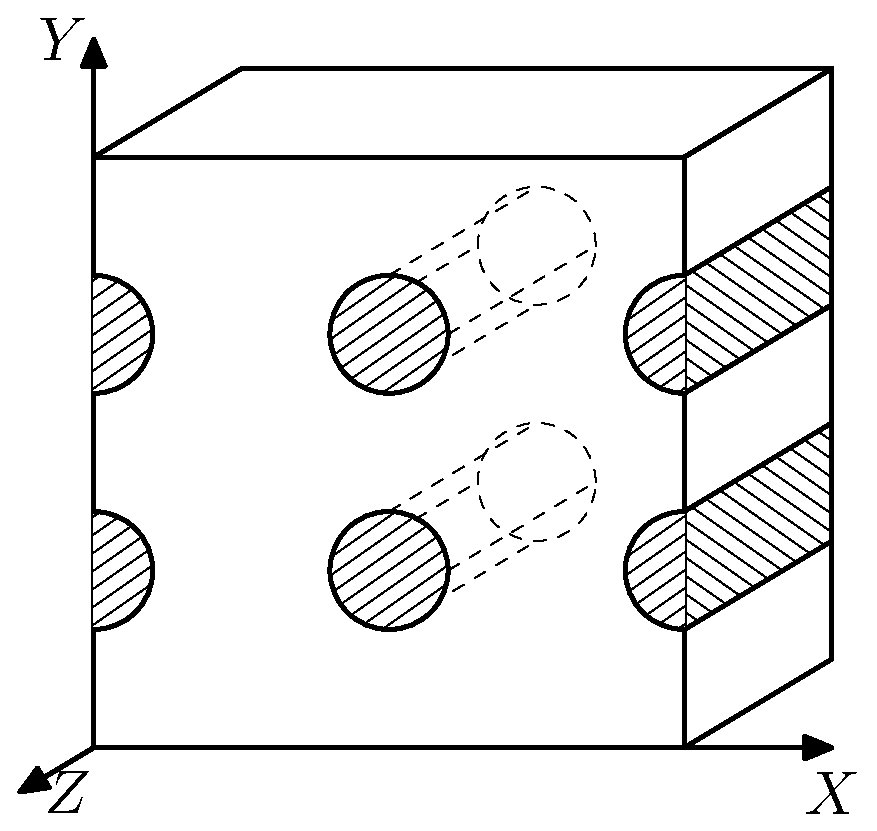
\includegraphics [scale=0.5] {images/two_period}
    \caption{2-периодчекая среда.} 
    \label{images:two_period}  
\end{figure}

3-периодические коомпозитные материалы (рис. 
\ref{images:three_period}
).  Физические свойства изменяются периодически вдоль всех трёх направлений.

\begin{equation}
    \begin{array}{ccc}
    \vec{a}_x = \left(\begin{array}{c}h_x\\0\\0\end{array}\right) & 
    \vec{a}_y = \left(\begin{array}{c}0\\h_y\\0\end{array}\right) & 
    \vec{a}_z = \left(\begin{array}{c}0\\0\\h_z\end{array}\right)
    \end{array}
\end{equation}

\begin{figure} [ht] 
    \center
    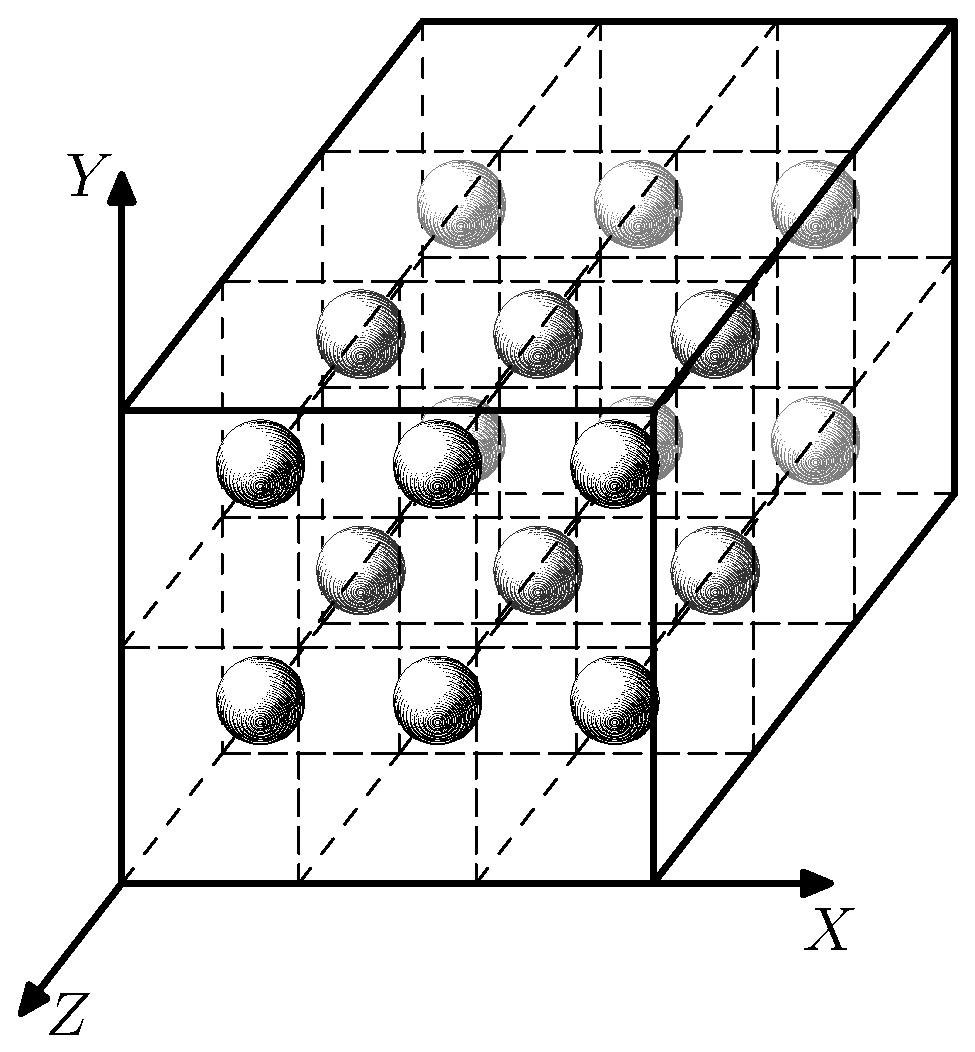
\includegraphics [scale=0.5] {images/three_period}
    \caption{3-периодчекая среда.} 
    \label{images:three_period}  
\end{figure}

Область в которой определяющие соотношения 
\ref{eq:BasicDefRelations}
непрерывны по координате будем называть компонентом композита.
Композит может иметь два и более компонента. 
Если композит двухкомпонентный, то один из компонентом можно называть связующим (матрицей), а другой включениями (в случае армированного композита арматурой, волокнами).

Функция
$\mathfrak{a}$,
входящая в правую часть соотношения
\ref{eq:BasicDefRelations},
непрерывна во всей области и не терпит разыв на границе раздела сред. 
В случае задачи упругости это соответствует идеальному контакту сред, входящих в состав композита, деформации не терпят разрыв на грнанице раздела сред.

Материльные функции изменяются с периодом порядка величины
$ \varepsilon \ll 1 $
. В таком случае при решении задачи напрямую численным методом придётся сильно измельчать сетку,
чотбы хотя бы несколько узлов попали на одно включение. 






\end{document}
